\externaldocument{../3/chapter_modeling}
\externaldocument{../4/chapter_algorithm}
\startchapter{Feature Prototype On Atlantis}
\label{chapter:newsol}
In this chapter, I present the design of the feature prototype of communication identification from the dual\_trace. This feature is implemented on Atlantis and is built on top of Atlantis' other features, such as ``memory reconstruction", ``function inspect" and ``views synchronization". Atlantis is an assembly trace analysis environment. It provides many powerful and novel features to assist assembly level execution trace analysis.\cite{huang2017atlantis} This prototype implemented some of the algorithms described in Chapter\ref{chapter:alo} as well as the user interfaces.

This prototype consists of four main components: 1) user setting for the function descriptors of the communication methods. 2) a view that can parallel display both traces in the dual\_trace. 3) two features: stream extraction and communication identification. 4) identification result navigation.

\section{User Setting of the Function Descriptors}\label{functionset}
In Section \ref{cdesc}, I defined a function descriptor as a set of function descriptions for a communication method. The communication identification approach can identify the communications described by the function descriptor from the dual\_trace.

However, the communication method description for a communication method can be different depends on the implementation solution of the communication method. Furthermore, there are so many communication methods in the real world, it is impossible to pre-define all of them for the users. Instead, a configuration file in Json format is provided for the users to define their communication methods of interest and the corresponding function descriptors. A default template is given for user reference, this default template is generated by Atlantis when it was launched and stored in the .tmp folder in the trace analysis project folder. The users can modify this template as to the communication methods of interest. The default template example can be find in Section\ref{funcset}.

The function descriptors in this setting file will be the input for the stream extraction and communication identification features. When the user use this two features, the list of the communication methods provided in the setting files will be presented to them. They can select one or more communication methods to be analysed. 

In the following subsections, function descriptor examples are presented as user reference to how to design their own function descriptor for a communication method.

\subsection{Communication Methods' Implementation in Windows}\label{windows}
Learning the implementation of a communication is necessary to obtain the function descriptor of the communication method.  In this section, I present the result of investigation about the implementation of the four communication methods: Named Pipe, Message Queue, TCP and UDP in Windows. In the investigation, I reviewed the Windows APIs of the communication methods and their example code. By doing so, I obtained the function descriptors of these methods can be designed by this investigation.

Windows API set is very sophisticated. Moreover, multiple solutions are provided to fulfil a communication method. It is impossible to enumerate all solutions for each communication method. I only investigated the most basic usage provided in Windows documentation. For each communication method, a function descriptor with a list of system function descriptions is provided for reference. The functions in the descriptors are supported in most Windows operating systems, such as Windows 8, Window 7. The provided function descriptor of a communication method should only be considered as an example for that communication method. With the understanding of this, it should be fairly easy to obtain the function descriptors for other solutions of that communication method or other communication methods. 

Note that, the instances of the descriptors only demonstrate Windows C++ APIs. But the idea of the function descriptor is generalizable to other operating systems with the effort of understanding the APIs of those operating systems.

\subsubsection{Windows Calling Convention}
The Windows calling convention is important to know in this research. The communication identification from dual\_trace in assembly level relies not only on the system function names but also the key parameter values. In the assembly level execution traces, the parameter values is captured in the memory changes and register changes of the instructions but without any information indicating which registers or memory addresses are holding this parameters. The calling convention tells us where the parameters are stored. So that we can find them in the memory state while emulate the execution of the trace. Calling Convention is various for operating systems and the programming language. I used dual-trace of Microsoft* x64 programs for case study in this research. The Microsoft* x64 example calling convention is listed in Appendix \ref{convention}.

\subsubsection{Named Pipes}
In Windows, a named pipe is a communication method for the pipe server and one or more pipe clients. The pipe has a name, can be one-way or duplex. Both the server and clients can read or write into the pipe.\cite{WinNamedpipe} In this work, I only consider one server versus one client communication. One server to multiple clients scenario can always be divided into multiple server and client communications thanks to the characteristic that each client and server communication has a separate conduit. The server and client are endpoints in the communication. We call the server ``server endpoint" while the client ``client endpoint".  The server endpoint and client endpoint of a named pipe share the same pipe name, but each endpoint has its own buffers and handles. 

There are two modes for data transfer in the named pipe communication method, synchronous and asynchronous.  Modes affect the functions used to complete the send and receive operation. Both descriptors for both synchronous mode and asynchronous mode are provided. The create channel functions for both modes are the same but with different input parameter value. The functions for send and receive message are also the same for both cases. However, the operation of the send and receive functions are different for different modes. In addition, an extra function \textit{GetOverlappedResult} is being called to check if the sending or receiving operation finish, the output message will be stored in the overlap structure whose memory address saved in the function's output parameter Overlap Structure Address. Table\ref{namesyn} is the function descriptor for synchronous mode while Table\ref{nameasyn} is the function descriptor asynchronous mode of Named pipe.

\begin{table}[H]
  \centering
  \caption{Function Descriptor for Synchronous Named Pipe}
  \label{namesyn}
  \begin{tabular}{|l|l|l|l|l|l|l|l|}
\hline
             \multirow{2}{*}{{\textbf{Name}}} & \multirow{2}{*}{{\textbf{Type}}} & \multicolumn{3}{c|}{\textbf{Input Parameter Description}} & \multicolumn{3}{c|}{\textbf{Output Parameter Description}} \\
              \cline{3-8} 
             & & \textbf{Name}& \textbf{Register} & \textbf{Addr/Val} & \textbf{Name}& \textbf{Register} &  \textbf{Addr/Val}  \\
             \hline
      CreateNamedPipe
       &open & FileName & RCX  & Addr &  Handle & RAX & Val\\
      \hline         
      CreateFile
       &open & FileName & RCX & Addr&  Handle & RAX & Val\\ 
      \hline              
      \multirow{2}{*}{WriteFile}
       &\multirow{2}{*}{send} &  Handle & RCX & Val & \multirow{2}{*}{Length} & \multirow{2}{*}{R9} & \multirow{2}{*}{Val}\\
        \cline{3-5} 
       & & SendBuf & RDX & Addr & & &\\
      \hline            
      \multirow{2}{*}{ReadFile}
       &\multirow{2}{*}{receive} &  Handle & RCX & Val& \multirow{2}{*}{Length} & \multirow{2}{*}{R9} & \multirow{2}{*}{Val}\\
        \cline{3-5} 
       & & RecvBuf & RDX  & Addr & & &\\
      \hline            
      CloseHandle &
       close &  Handle & RCX & Val & & &\\
      \hline            
      DisconnectNamedPipe &
      close &  Handle & RCX & Val & & &\\
      \hline               
  \end{tabular}
\end{table}

\begin{table}[H]
  \centering
  \caption{Function Descriptor for Asynchronous Named Pipe}
  \label{nameasyn}
\begin{tabular}{|l|l|l|l|l|l|l|l|}
\hline
             \multirow{2}{*}{{\textbf{Name}}} & \multirow{2}{*}{{\textbf{Type}}} & \multicolumn{3}{c|}{\textbf{Input Parameter Description}} & \multicolumn{3}{c|}{\textbf{Output Parameter Description}} \\
              \cline{3-8} 
             & & \textbf{Name}& \textbf{Register} & \textbf{Addr/Val} & \textbf{Name}& \textbf{Register} &  \textbf{Addr/Val}  \\
             \hline
      CreateNamedPipe
       &open & FileName & RCX  & Addr &  Handle & RAX & Val\\
      \hline         
      CreateFile
       &open & FileName & RCX & Addr&  Handle & RAX & Val\\ 
      \hline              
      \multirow{2}{*}{WriteFile}
       &\multirow{2}{*}{send} &  Handle & RCX & Val & \multirow{2}{*}{Length} & \multirow{2}{*}{R9} & \multirow{2}{*}{Val}\\
        \cline{3-5} 
       & & SendBuf & RDX & Addr & & &\\
      \hline            
      \multirow{2}{*}{ReadFile}
       &\multirow{2}{*}{receive} &  Handle & RCX & Val& \multirow{2}{*}{Length} & \multirow{2}{*}{R9} & \multirow{2}{*}{Val}\\
        \cline{3-5} 
       & & RecvBuf & RDX  & Addr & & &\\
      \hline    
           GetOverlappedResult &
       receive &  Handle & RCX & Val &OverlapStruct &RDX & Addr\\
      \hline     
      CloseHandle &
       close &  Handle & RCX & Val & & &\\
      \hline            
      DisconnectNamedPipe &
      close &  Handle & RCX & Val & & &\\
      \hline               
  \end{tabular}  
\end{table}

\subsubsection{Message Queue}
Similar to Named Pipe, Message Queue's implementation in Windows also has two modes, synchronous and asynchronous. Moreover, the asynchronous mode further divides into two operations, one with callback function while the other without. With the callback function, the callback function would be called when the send or receive operations finish. Without callback function, the general function \textit{MQGetOverlappedResult} should be called by the endpoints to check if the message sending or receiving operation finish, the parameter in RCX of this function call is a structure consist of the handle as an input parameter and the overlap structure as an output parameter. Table\ref{msmqsynfunctions} is the function descriptor for synchronous mode while Table\ref{msmqasynfunctions} is the function descriptor for the asynchronous mode without callback. With callback function situation is not elaborated here.

\begin{table}[H]
  \centering
  \caption{Function Descriptor for Synchronous Message Queue}
  \label{msmqsynfunctions}
\begin{tabular}{|l|l|l|l|l|l|l|l|}
\hline
             \multirow{2}{*}{{\textbf{Name}}} & \multirow{2}{*}{{\textbf{Type}}} & \multicolumn{3}{c|}{\textbf{Input Parameter Description}} & \multicolumn{3}{c|}{\textbf{Output Parameter Description}} \\
              \cline{3-8} 
             & & \textbf{Name}& \textbf{Register} & \textbf{Addr/Val} & \textbf{Name}& \textbf{Register} &  \textbf{Addr/Val}  \\
             \hline
      MQOpenQueue
       &open & QueueName & RCX  & Addr &  Handle & RAX & Val\\
      \hline                     
      \multirow{2}{*}{MQSendMessage}
       &\multirow{2}{*}{send} &  Handle & RCX & Val &  &  & \\
       \cline{3-5}
      & & MessStruct& RDX&Addr &  &  & \\
      \hline            
      MQReceiveMessage
       &receive&  Handle & RCX & Val& MessStruct& RDX&Addr\\
      \hline       
      MQCloseQueue &
       close &  Handle & RCX & Val & & &\\
      \hline                          
  \end{tabular}   
\end{table}

\begin{table}[H]
  \centering
  \caption{Function Descriptor for Asynchronous Message Queue}
  \label{msmqasynfunctions}
\begin{tabular}{|l|l|l|l|l|l|l|l|}
\hline
             \multirow{2}{*}{{\textbf{Name}}} & \multirow{2}{*}{{\textbf{Type}}} & \multicolumn{3}{c|}{\textbf{Input Parameter Description}} & \multicolumn{3}{c|}{\textbf{Output Parameter Description}} \\
              \cline{3-8} 
             & & \textbf{Name}& \textbf{Register} & \textbf{Addr/Val} & \textbf{Name}& \textbf{Register} &  \textbf{Addr/Val}  \\
             \hline
      MQOpenQueue
       &open & QueueName & RCX  & Addr &  Handle & RAX & Val\\
      \hline                     
      \multirow{2}{*}{MQSendMessage}
       &\multirow{2}{*}{send} &  Handle & RCX & Val &  &  & \\
       \cline{3-5}
      & & MessStruct& RDX&Addr &  &  & \\
      \hline            
      MQReceiveMessage
       &receive&  Handle & RCX & Val& MessStruct& RDX&Addr\\
      \hline    
      MQGetOverlapResult &
       receive &  Handle & RCX & Addr & Overlapstr& RCX&Addr\\
      \hline      
      MQCloseQueue &
       close &  Handle & RCX & Val & & &\\
      \hline                          
  \end{tabular}   
\end{table}


    
\subsubsection{TCP and UDP}
In Windows programming, these two methods shared the same set of APIs regardless the input parameter values and operation behaviour are different. In Windows socket solution, one of the two endpoints is the server while the other one is the client. Table \ref{tcpupdfunctions} is the function descriptor for UDP or TCP communication. 

\begin{table}[H]
  \centering
  \caption{Function Descriptor for for TCP and UDP}
  \label{tcpupdfunctions}
\begin{tabular}{|l|l|l|l|l|l|l|l|}
\hline
             \multirow{2}{*}{{\textbf{Name}}} & \multirow{2}{*}{{\textbf{Type}}} & \multicolumn{3}{c|}{\textbf{Input Parameter Description}} & \multicolumn{3}{c|}{\textbf{Output Parameter Description}} \\
              \cline{3-8} 
             & & \textbf{Name}& \textbf{Register} & \textbf{Addr/Val} & \textbf{Name}& \textbf{Register} &  \textbf{Addr/Val}  \\
             \hline
      socket
       &open &  &   &  &  Socket & RAX & Val\\
      \hline
      bind
       &open & Socket &  RCX & Val &  ServerAddrAndPort & RDX & Addr\\
      \hline   
            connect
       &open & Socket &  RCX & Val &  ServerAddrAndPort & RDX & Addr\\
      \hline   
     accept
       &open &  ListenSocket & RCX & Val & ConnectSocket & RAX & Val\\
      \hline                    
      \multirow{2}{*}{send}
       &\multirow{2}{*}{send} &  Handle & RCX & Val &  &  & \\
       \cline{3-5}
      & & SendBuf& RDX&Addr &  &  & \\
      \hline            
      recv
       &receive&  Handle & RCX & Val& RecvBuf& RDX&Addr\\
      \hline      
      closesocket &
       close &  Handle & RCX & Val & & &\\
      \hline                          
  \end{tabular}    
\end{table}

\section{Parallel Editor View For Dual\_Trace}
The dual\_trace consist of two execution traces which are interacting with each other. Presenting them in the same view makes the analysis for the user much easier. To open parallel editor view, the user need to open one trace as the normal one and the other as the dual\_trace of the opened one. A new menu option in the project navigation view are added to open the second trace as the dual\_trace of the active trace. The implementation of the parallel editor take the advantage of the existing SWT of Eclipse plug-in development. The detail of the implementation can be found in Appendix \ref{paralleleditor}. Figure \ref{opendualtracemenu} shows this menu option and Figure \ref{paralleleditor} shows the parallel editor view.

\begin{figure}[H]
\centerline{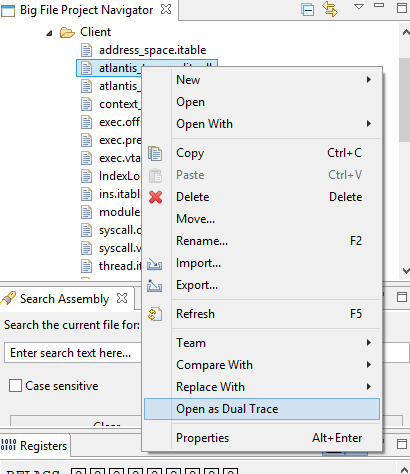
\includegraphics[scale=0.4]{Figures/opendualtracemenu}}
 \caption{Menu Item for opening Dual\_trace}
\label{opendualtracemenu}
\end{figure}

\begin{figure}[H]
\centerline{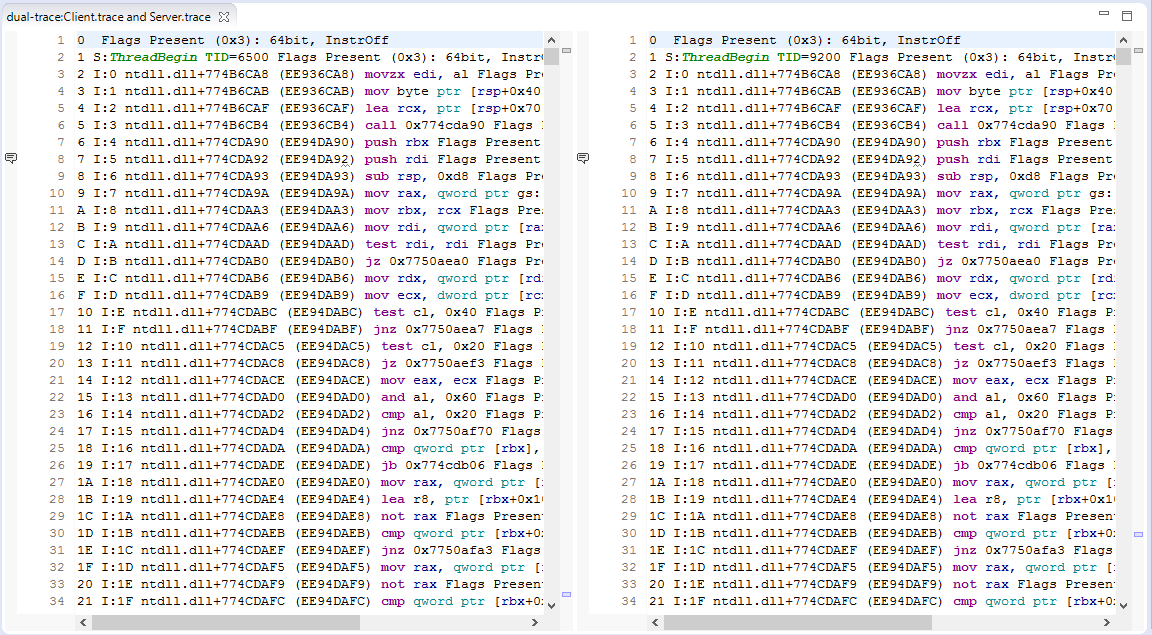
\includegraphics[scale=0.6]{Figures/paralleleditor}}
 \caption{Parallel Editor View}
\label{paralleleditor}
\end{figure}

\section{Identification Features}
I implemented two features. The first one is stream extraction corresponding to the stream extraction algorithm presented in Chapter\ref{chapter:alo} for both traces in the dual\_trace. The other one is the communication identification corresponding to the overall communication process discussed in Chapter\ref{chapter:alo}. The implementation of these two features relies on the existing ``function inspect" feature of Atlantis. The called functions' name can be inspected  by  search of the symbolic name in the executable binary or any DLLs which used by the program at the time when it is traced. By importing the DLLs and executable binary, Atlantis can recognize the function call from the execution trace by the function names. Therefore the corresponding Dlls or executable binaries for both traces in the dual\_trace have to be loaded into Atlantis before conducting the identification.

A new menu ``Dual\_trace Tool" with three menu options is designed for these two features. In this menu, ``Stream Identification" is for the operation of stream extraction and ``Communication Identification" is for the operation of communication identification. For both of these two operation ``Load Library Exports" has to be run before for both traces. Currently, the ``Load library export"  operation can only load libraries for the trace in the active editor. So ``Load library export"  in the menu has to be run twice separately for each trace of the dual\_trace.  Figure\ref{dualtracetoolmenu} shows this new menu in Atlantis. When the user perform ``Stream Identification" or ``Communication Identification", there will be a prompt dialog as shown in Figure \ref{methods} which asks the user what communication methods they want to analyse from the dual\_trace. This list is provided by the configuration file I mention in Section \ref{functionset}. The user can select one or multiple methods. 

\begin{figure}[H]
\centerline{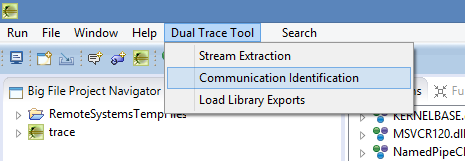
\includegraphics{Figures/dualtracetoolmenu}}
 \caption{Dual\_trace Tool Menu}
\label{dualtracetoolmenu}
\end{figure}

\begin{figure}[H]
\centerline{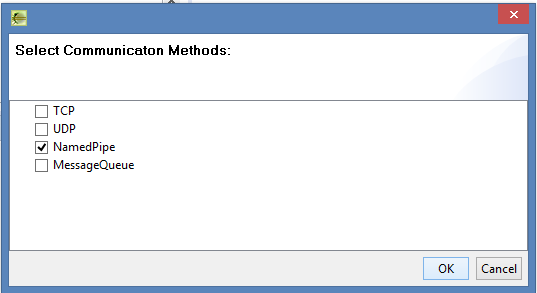
\includegraphics[scale=0.8]{Figures/methods}}
 \caption{Prompt Dialog for Communication Selection}
\label{methods}
\end{figure}

A new view named ``Communication" is designed for presenting the result of the extracted streams and the identified communications. Since the user can have multiple selection for communication methods of interest, the output identification result contains all the identified communications or streams of all selected communication methods and the results are clustered by methods. There are two sub tables in this view, the left one is for presenting the extracted the streams result while the left one is for presenting communication identification result. The reason for putting this two result in the same view is for easy access and comparison of the data for the users. Figure \ref{idenview} shows this view with result data in it. Each time when the user rerun the features the result in the corresponding table will be refreshed to show only the latest identification result. But the other table will not be affected. For example, if the user run the ``Stream Identification" feature first, the stream result will show on the left table of the view. And then the user run the ``communication Identification", the communication identification result will be shown on the right table while the left one still holding the last stream result.

\begin{figure}[H]
\centerline{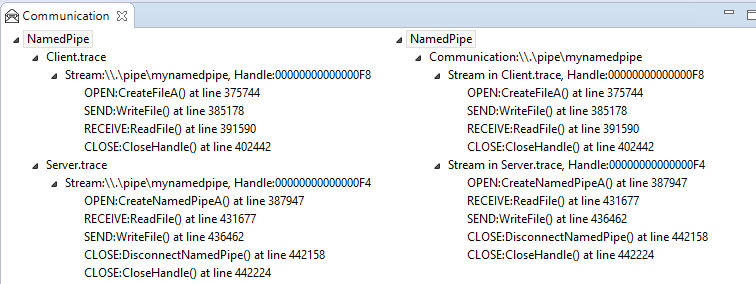
\includegraphics[scale=0.7]{Figures/idenview}}
 \caption{Communication View for Result}
\label{idenview}
\end{figure}

\section{Result Navigation}
Atlantis is a analysis environment that has various views to allow user access to different information from the trace, such as the memory and register state of the current instruction line. Moreover, these views synchronize automatically with the editor view. These functionality and information also benefit the communication analysis of the dual\_trace. Providing the user a way to navigate from the result to the traces in the editors allows them to take advantage of the current existing functionality of Atlantis and make their analysis of the dual\_trace more efficient.

In the result list, each event entry is corresponding to a function call. The functions were called at function call line and all the inputs of the function calls can be recovered from the memory state of this instruction line. The functions returned at the return instruction lines, all the outputs of the function calls can be recovered in the memory state of the the return instruction line. From the event entries, this implementation provide two different ways for the user to navigate back to where the function begins and ends. When the user ``double click" on an entry, it will bring the user to the start line of the function in the corresponding trace editor. When the the right click on the event entry, a prompted menu with the option ``Go To Line of Function End" will show up as in Figure \ref{gotoend}. Clicking on this option will bring the user to the return line of this function in the trace editor. All other views update immediately with this navigation. 

\begin{figure}[H]
\centerline{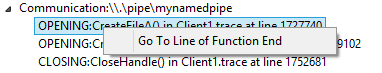
\includegraphics{Figures/gotoend}}
 \caption{Right Click Menu on Event Entry}
\label{gotoend}
\end{figure}

Moreover, the ``remove" option as shown in Figure \ref{remove} in the right click menu on the ``stream“ or ``communication" entries is provided for the user to remove the selected ``stream" or ``communication" entry. This provides the user the flexibility to get rid of the data that they don't care.

\begin{figure}[H]
\centerline{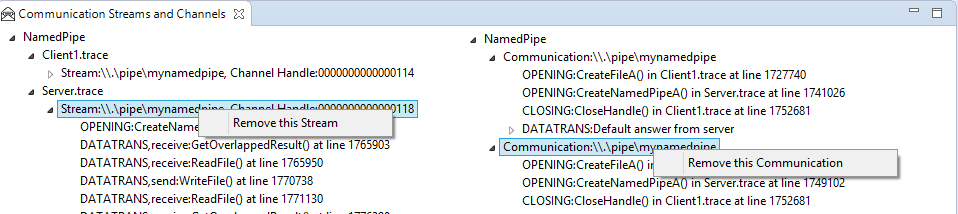
\includegraphics[scale=0.7]{Figures/remove}}
 \caption{Right Click Menu on Event Entry}
\label{remove}
\end{figure}

